\subsection{Screening Prioritisation}


Screening is assessing a document to determine if it is relevant or not relevant to the search query. Screening prioritisation ranks documents such that documents relevant to the search query are above those that are not. Consider the following hypothetical scenario. You have 20 documents that you need to screen. If you do not prioritise (i.e. rank) the documents, you would have to look at all twenty documents to find those documents if you order these documents with the more relevant ones first. Theoretically, the minimum number of documents a screener must consider equals the total number of relevant ones.

Many approaches to automating screening prioritisation have been proposed. Early work focused on the statistical properties of words contained within the title and abstract.






Automatic term recognition (ATR) operates in two phases. First, the titles and abstracts of eligible studies are provisionally analysed, and a list of terms, together with the score which indicates their relative importance, is obtained. Second, the top 100 terms are used to search the unlabelled documents with search terms weighting to the score given from the first. 

The study demonstrated that using ATR in the Choice Architecture (CA) review led to an observed inclusion rate (OIR) to baseline inclusion rate (BIR) ratio of 10.1. This means that ATR performed approximately 10 times better than screening a random sample of records (a proxy for conventional screening methods). This equates to a proportionate reduction in manual screening workload of 90.1


Automatic classification













Technology-Assisted Review (TAR), also known as Computer-Assisted Review or Predictive Coding, is a process that uses machine learning to assist in document review tasks. In the context of SRs, the TAR applies active learning (AL) principles to streamline the selection process of titles and abstracts to screen. By iteratively training a machine learning model on human-labelled examples, TAR can prioritise potentially relevant documents for expert review, significantly reducing manual workload and, in some cases, exceeding human ability \cite{grossman_technology-assisted_2010}. TAR has been successfully applied in Law disclosure, \hl{x y and z}.

\subsubsection{Active Learning}



Deep learning models generally excel when trained on vast amounts of labelled data. This presents a significant challenge during the early stages of SR search, where the initial pool of labelled documents is often very limited. Active learning (AL) offers a solution by intelligently selecting the most informative unlabeled documents for manual labelling by a human expert. This iterative process aims to substantially improve model performance while minimising the time and effort required for labelling. A typical AL workflow selects a batch of unlabeled samples based on their potential to improve the model. These selected samples are then labelled and incorporated into the growing training dataset. The model is subsequently retrained using this expanded dataset, leading to improved classification and ranking accuracy. The core principle behind AL is to balance exploring uncertain or ambiguous documents (exploration) and exploiting documents that are likely to be highly relevant (exploitation). This approach enhances the model's ability to rank documents accurately, making the SR process more efficient and effective.

Different approaches have been taken to AL, such as membership query synthesis \cite{angluin_queries_1988}, stream-based selective \cite{akinseloyin_novel_2024} and pool-based sampling \cite{lewis_sequential_1994}. These approaches are delineated on how much of the unlabelled dataset a model can access when utilising a policy for selecting data points to be labelled. In pool-based sampling, the entire unlabelled dataset is evaluated in choosing the batch to be labelled. In stream-based selective sampling, data points are evaluated one at a time, and a model decides on the fly to label them. Synthetic data are generated from an underlying natural distribution in membership query synthesis. During the title and abstract screening substage, pool-based sampling is most appropriate as the unlabeled dataset is known beforehand. Figure \ref{fig:pool_based_query} outlines the AL cycle with pool-based querying.

\begin{figure}
\centering
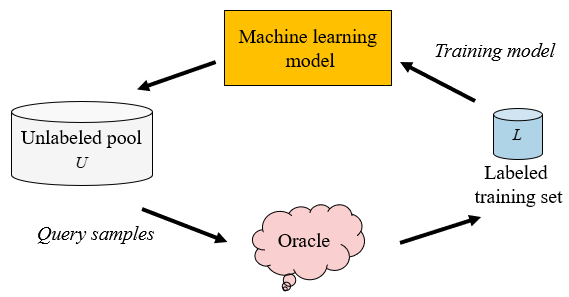
\includegraphics[width=0.5\linewidth]{images/pool_based_strategy.png}
\caption{Overview of a pool-based query strategy for AL, replicated\cite{ren_survey_2021}}.
\label{fig:pool_based_query}
\end{figure}




The AL process can be described as follows: a sampling policy $\pi$ intelligently selects the most informative samples  $\mathbf{T}_{C,i}$ from an unlabelled dataset $\mathbf{T}_{U,i}$.  These samples are passed to an oracle $O$ for labelling and then added to a growing known dataset $\mathbf{T}_{K,i}$. A classifier is trained on this labelled dataset and used to rank the remaining unlabeled samples in $\mathbf{T}_{U,i}$, often based on the classifier's uncertainty or expected model improvement. This iterative process repeats, intending to improve the classifier's performance with each labelling round until a predefined stopping criterion is met. The oracle ($O$) within SRs denotes a human-verified label resulting from screening potential research for inclusion within the SR within the title and abstract screening stage. More concretely, $O$ can be considered a function $O(x) = y$ where $X$ is a representation (i.e. if a human was reviewing a title and abstract, or a representation of the title and abstract for automated approaches), and $y$ is the assigned category (included or excluded). It is assumed that for each datapoint ($x$), $O$ provides a single judgement ($y$), which is always correct and do not concern ourselves with any potential intercoder agreement or bias within that decision process \cite{artstein_survey_2008}.




\begin{table*}[t]
    \centering
    \footnotesize

    \begin{tabular}{|c|c|>{\raggedright\arraybackslash}p{11cm}|}
        \hline
        \textbf{Notation}    & \textbf{Explanation}                            & \textbf{Notes}                                                                                \\
        \hline
        \(\textbf{T}\)       & Total dataset                                   & e.g. Research gathered after Identification phase of the selection process.                   \\
        \hline
        \(i\)                & Iteration                                       & A single cycle within the active learning process.                                            \\
        \hline
        \(\textbf{T}_{K,i}\) & Known datapoints per iteration                  & e.g. research that has been screened by a reviewer                                            \\
        \hline
        \(\textbf{T}_{U,i}\) & Unknown datapoints per iteration                & e.g. research that has not been screened by a reviewer                                        \\
        \hline
        \(\textbf{T}_{C,i}\) & A subset of \(\textbf{T}_{U,i}\) to be labelled & chosen by a policy, datapoints to be screened by a reviewer.                                  \\
        \hline
        $\pi$                & Policy                                          & How \(\textbf{T}_{U,i}\) is selected, e.g. uncertainty, random, certainty, diversity sampling \\
        \hline
        O                    & Oracle                                          & Often a domain expert, who assigns labels to unscreened research.                             \\
        \hline
        \(T_R\)              & Total Relevant Documents                        & All research that should be included in a systematic review.                                  \\
        \hline
        \(T_{IR}\)           & Total Irrelevant Documents                      & All research that should not be included in a systematic review.                              \\
        \hline
    \end{tabular}
    \caption{Notation used for active learning within this review}
    \label{tab:notation}
\end{table*}






The AL approach has, however, shortcomings when applying it to SRs.
\hl{Waiting until a minimum number of documents has been assessed has several disadvantages. Firstly information gathered in the early phases is not incorporated into the ranking. Secondly, it requires the actual search phase to be delayed; minimum number of relevant studies are present in the document collection; and finally.....}



However, the truly minimise screening ...


we would want to move to a scenario where minimal expert screening is sought from research returned from the identification phase, whose screening can then be safely extrapolated to a larger pool.